\chapter{Анализ структурных схем и способов проектирования главного тракта приема сверхширокополосных сигналов}

\section{Главный тракт приема сверхширокополосных сигналов}
\subsection{Анализ современных трактов приема}

\chapter*{Постановка задачи}
Характеристики приведены в Табл.\ref{tab:Parameters}.
\begin{table}[h]
	\caption[Характеристики разрабатываемого АЦП]{Характеристики разрабатываемого АЦП}
	\label{tab:Parameters}
	\centering
	\begin{tabular}{rrr}
		\toprule
		\textbf{Параметр}      & \textbf{Значение} & \textbf{Единица измерения}\\
		\midrule
		\(N\)                 &   14      & Бит\\
		\(F_{clk}\)           &   250     & МГц\\
		\(V_{FS}\)            &   1.2     & В\\
		\(V_{CM_{in}}\)                   &   600     & мВ\\
		\(FPBW\) (Full Power Bandwidth)   & 750 & МГц\\
		\bottomrule
	\end{tabular}
\end{table}

\section{Современные методы проектирования и структуры сверхширокополосных малошумящих усилителей}

Основными параметрами МШУ являются:
\begin{itemize}
	\item Коэффициент шума;
	\item Коэффициент усиления;
	\item Точка одноцебельной компрессии;
	\item Точка интермодуляции (перехвата) третьего порядка;
	\item Потребляемая мощность.
\end{itemize}

Согласно формуле Фрииса \eqref{eq:friise} основной вклад в шумовую характеристику приемного тракта вносит первый усилительный каскад.

\begin{equation}
F_{total} = F_1 + \frac{{F_2 - 1}}{G_1} + \frac{{F_3 - 1}}{G_1 G_2} + \frac{F_4 - 1}{G_1 G_2 G_3} + ... + \frac{F_N - 1}{\prod\limits_{N=1} G_N},
\label{eq:friise}
\end{equation}
где \(F_{total}\) -- суммарный коэффициент шума приемного тракта, \(F_N\) -- коэффициент шума \textit{N}-го каскада, \(G_N\) -- коэффициент усиления \textit{N}-го каскада.

Из выражения \eqref{eq:friise} следует, что для удовлетворения требований к МШУ, перечисленных выше, необходимо снижать коэффициент шума каждого каскада при одновременном увеличении коэффициента усиления. Исходя из данного наблюдения возникает противоречие, т.к. для повышения коэффициента усиления необходимо увеличивать ток потребления усилителя. При увеличении коэффициента усиления, ухудшается линейность усилителя, следовательно, уменьшается динамический диапазон устройства. При попытке улучшить линейность усилителя, уменьшается коэффициент усиления каждого каскада, в следствии чего возрастает коэффициент шума.

Из-за подобной связности какого-либо параметра с любым другим практически не существует универсальных способов и схем, позволяющих разработать усилитель удовлетворяющий всем требуемым характеристикам технического задания.

\subsection{Источники возникновения шумов в полупроводниковых устройствах}

\subsection{Принцип действия широкополосного малошумящего усилителя}

\subsection{Входное согласование по мощности}
Качество входного согласования выражается в значении отраженной мощности или возвратных потерь, которые для входного сопротивления МШУ \(Z_{in}\) и сопротивления источника \(R_S\) определяются как \eqref{eq:gamma}

\begin{equation}
\label{eq:gamma}
\Gamma = {\Bigg| \frac{Z_{in} - R_S}{Z_{in} + R_S} \Bigg|}^2
\end{equation}

\subsection{Первый каскад МШУ}
Так как основное влияние на шумовые характеристики оказывает первый каскад усиления, тогда к проектированию данного узла необходимо подойти максимально ответственно.

В качестве усилительного каскада могут применяться схемы включения транзистора:
\begin{itemize}
	\item Общий эмиттер (общий исток);
	\item Общая база (общий затвор);
	\item Каскодная схема -- общий эмиттер-общая база (общий исток-общий затвор).
\end{itemize}

При работе на частотах диапазона Ka (27 -- 40 ГГц) и выше, каскодная схема и общая база используются реже из-за ухудшающихся шумовых характеристик и, в случае каскода, повышенной промежуточной емкостью в узле соединения двух транзисторов, что приводит к значительному ухудшению усилительных свойств каскада.

\subsection{МШУ с дифференциальным выходом}

\subsection{Возникновение и методы снижения влияния нелинейных эффектов}

\section{Сверхширокополосные смесители}

\subsection{Сверхширокополосные смесители в интегральном исполнении}

\subsection{Шумы в полупроводниковых смесителях}

\chapter{Постобработка}
\section{Усилитель с регулировкой коэффициента усиления}

\subsection{Основные структуры}

\section{Широкополосный активный фазовращатель}

\section{Устройства выборки-хранения}
Определим мощность шумов квантования идеального АЦП с разрядностью \(N\) и размахом полной шкалы \(V_{FS}\)
\[ {P_{q}}^2 = \frac{\Delta^2}{12}\]
если \(\Delta = \dfrac{V_{FS}}{2^N}\), тогда \( {P_q}^2 = 223.52~\mathrm{pW} \).

\begin{figure}[ht]
	\centering
	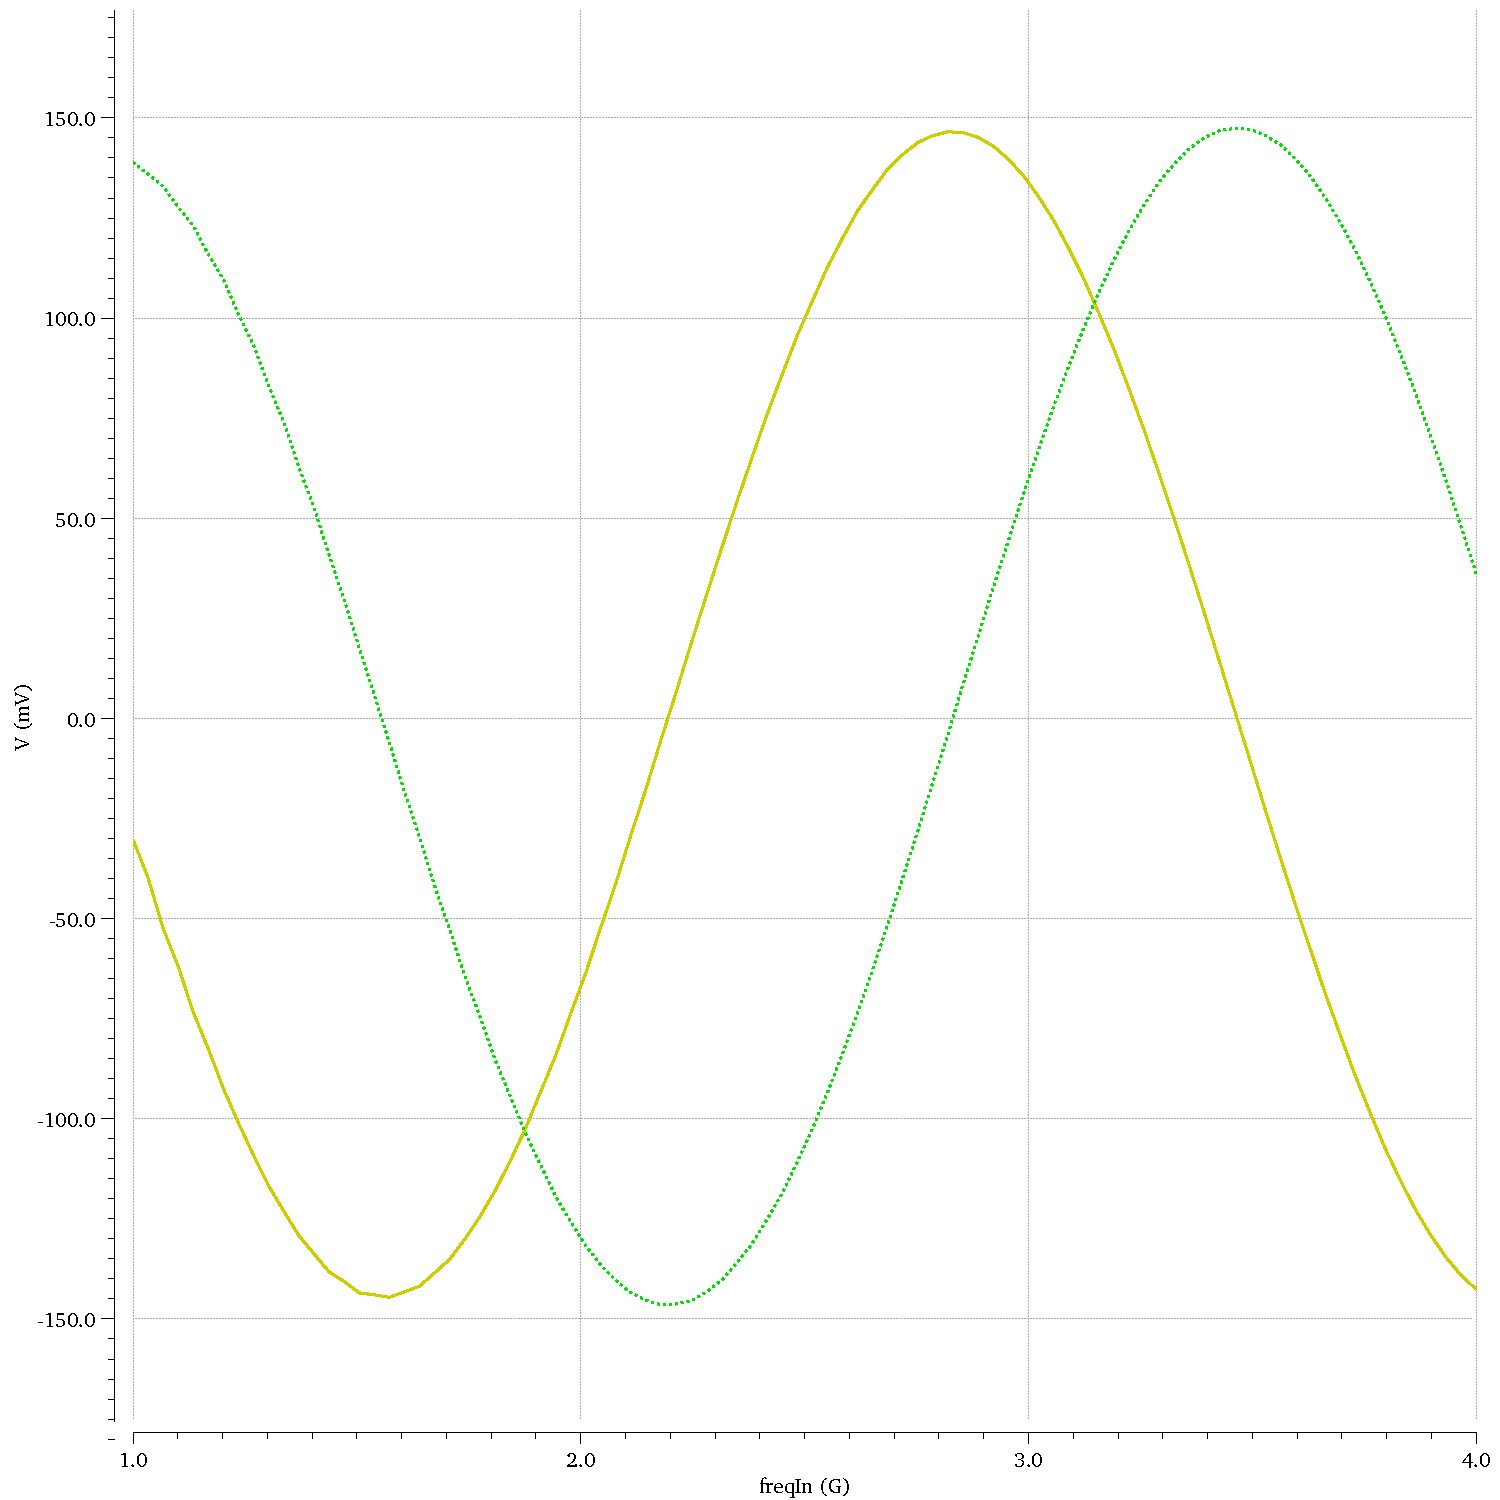
\includegraphics[width=0.8\linewidth]{discr_out}
	\caption{Квадратурный сигнал на выходе дискриминатора}
	\label{fig:discr_out}
\end{figure}

\begin{figure}[ht]
	\centering
	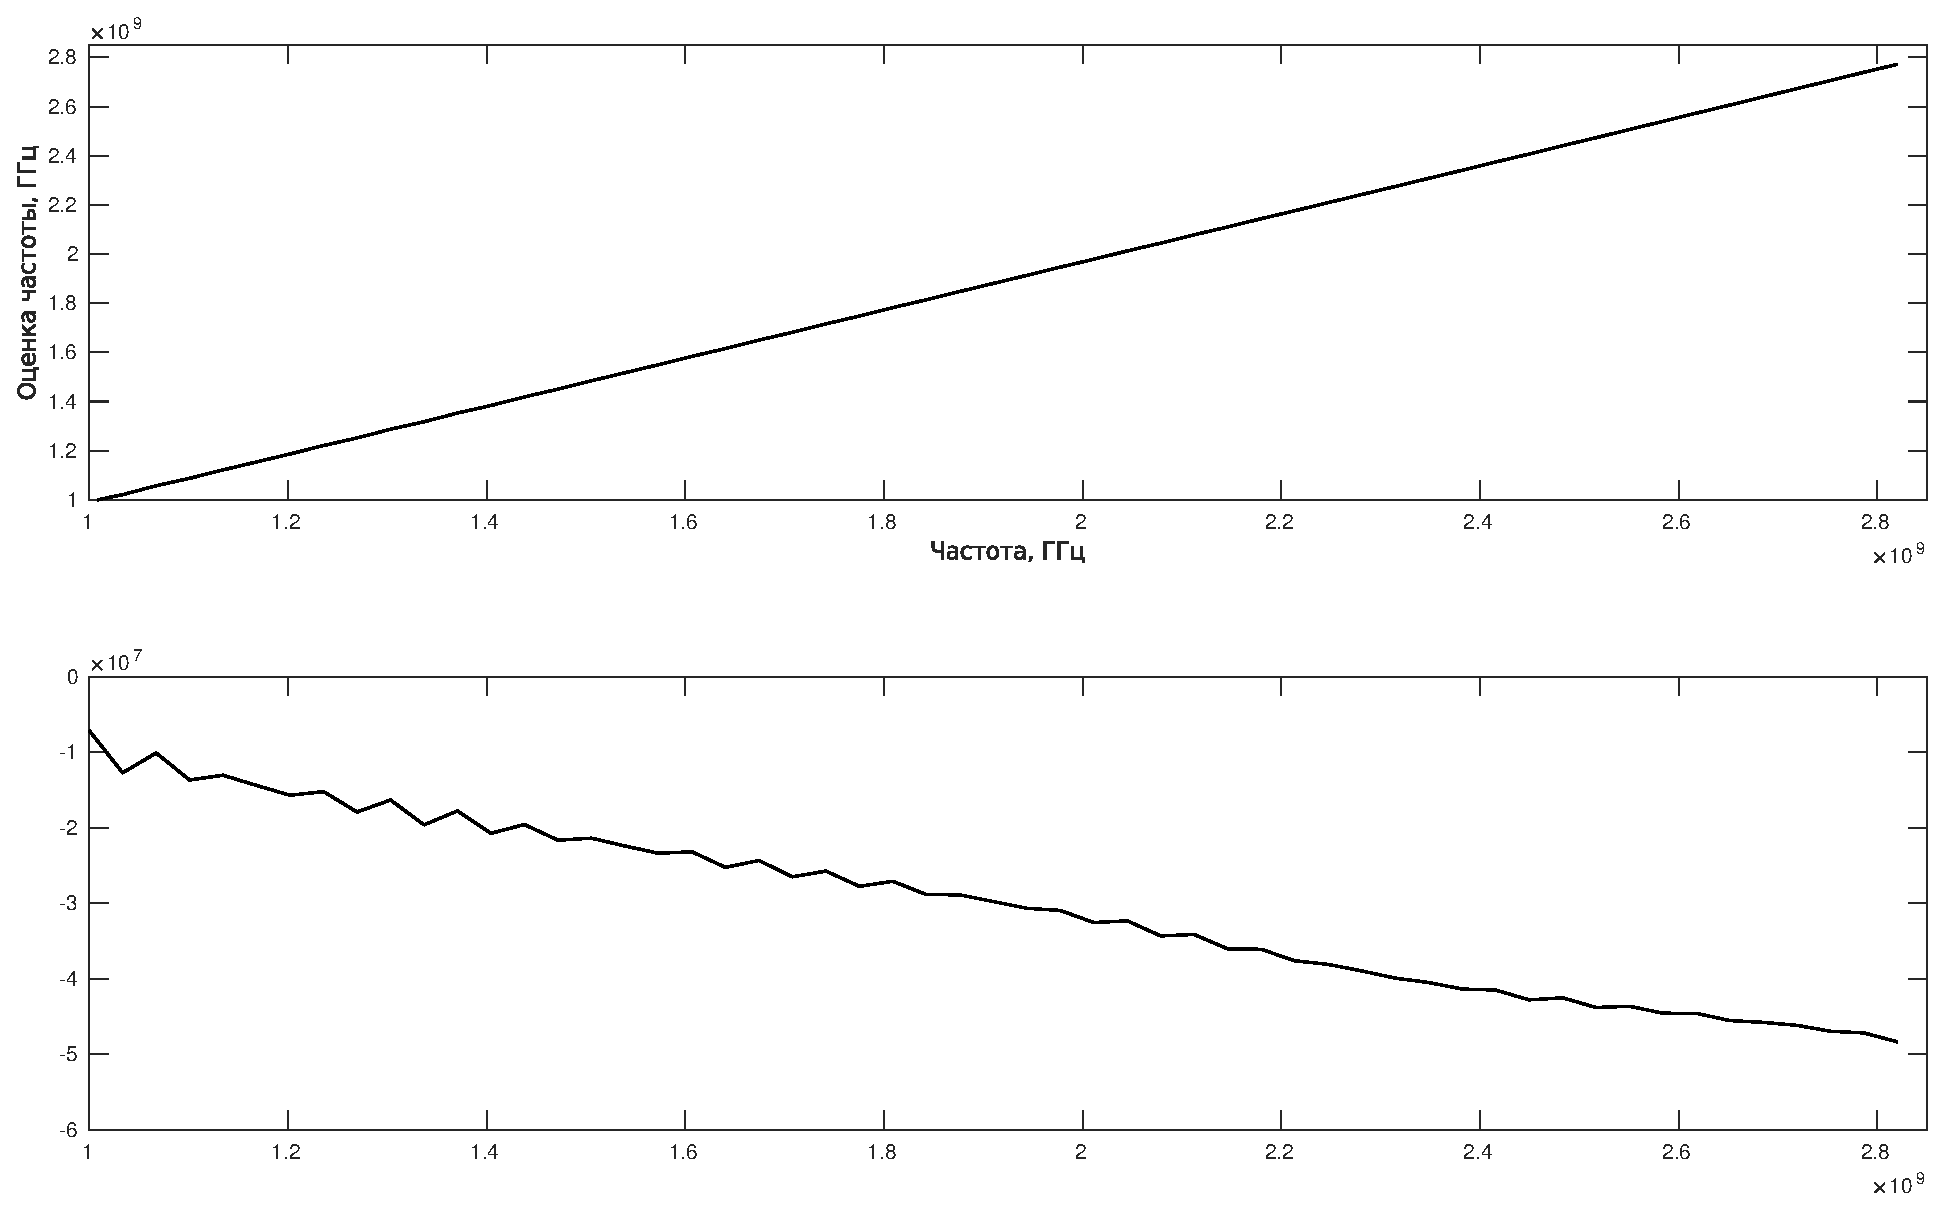
\includegraphics[width=0.8\linewidth]{SurfacePlot.eps}
	\caption{Квадратурный сигнал на выходе дискриминатора}
	\label{fig:discr_out2}
\end{figure}

\chapter{Схемотехнический расчет СФ-блоков}

\section{Устройство выборки-хранения в технологическом процессе кремний-германий 55 нм}
УВХ построено на базе МОП ключа Q1 с цепью смещения напряжения затвора \(V_{gs1}\), позволяющей снизить нелинейность ключа, возникающую из-за неполного <<закрытия>> или <<открытия>> канала.

\begin{figure}[ht]
	\centering
	\begin{circuitikz}[american, scale=1, transform shape]
		\ctikzset{tripoles/mos style/arrows}
		\ctikzset{bipoles/thickness=2}
		\ctikzset{tripoles/pmos style/emptycircle}
		\def\killdepth#1{{\raisebox{0pt}[\height][0pt]{#1}}} \path (0,0) -- (2,0); % bounding box
		\draw (0,0) node[nmos,rotate=-90](Q1){\rotatebox{90}{Q1}};
		\draw (Q1.D) to [short, l=Out, -] ++(2,0) to[C, l2^=$C_h$ and 4 pF]
		++(0,-1) node[ground](GND){};    ++(0,-1) node[ground](GND){};
		
		
		\draw ++(-3,0) coordinate(in) node[left](vi1){$v_i=v_1$} [short, l=Input, o-] to (Q1.S);
		\draw (in) ++(2,0) [short, *-] to ++(0,2) node[nmos, rotate=-90, anchor=D](Q2){\rotatebox{90}{Q2}};
		\draw (Q2.G) [short, -] to (Q2.G -| Q1.G) [short,-] to (Q1.G);
		\draw (Q2.S) node[nmos, rotate=-90, anchor=D](Q3){\rotatebox{90}{Q3}};
		\draw (Q3.D) [short, *-] to [C] ++(0, 4) coordinate(temp);
		\draw (temp) node[pmos, bulk, rotate=90, anchor=D, xscale=-1](Q4){\scalebox{1}[-1]{\rotatebox{90}{Q4}}};
		\draw (Q4.S) [short, -, l_=VDD] to ++(-1,0) coordinate(VDD);
		\draw (Q4.bulk) [short, -*] to (Q4.D);
		\draw (Q4.D) node[pmos, bulk, rotate=90, anchor=S, xscale=1](Q5){\rotatebox{-90}{Q5}};
		\draw (Q5.bulk) [short, -] to (Q5.S);
		\draw (Q5.D) [short, -] to (Q5.D -| Q1.G) to (Q2.G -| Q1.G);
		\node [circ] at (Q2.G -| Q1.G){};
		\draw (Q5.D -| Q1.G) node[nmos, anchor=S, rotate=-90, xscale=-1](Q6){\scalebox{1}[-1]{\rotatebox{-90}{Q6}}};
		\node [circ] at (Q5.D -| Q1.G){};
		\draw (Q6.D) [short, l=GND, -] to ++(1,0) coordinate(GND);
		\draw (Q4.G) [short, -] to (Q4.G -| Q6.S) to (Q6.S);
		
		\draw (Q3.G) [short, -, l_=clk] to (Q3.G -| VDD);
		\draw (Q3.S) [short, -, l=GND] to ++(-1,0);
		
		\draw (Q5.G) [short, -] to (Q6.G);
		\node [circ] at (Q6.G){};
		\draw (Q6.G) [short,-,l=clk] to (Q6.G -| GND);
		
		%COOOOOORDS
		%\path (temp) \coord(temp);
	\end{circuitikz}
	
	\caption{Схема устройства выборки-хранения}
	\label{ct:bootstrapped_switch}
\end{figure}

\begin{figure}[ht]
	\centering
	\begin{circuitikz}[american, scale=1, transform shape]
		\def\killdepth#1{{\raisebox{0pt}[\height][0pt]{#1}}} \path (0,0) -- (2,0); % bounding box
		\ctikzset{transistors/arrow pos=end}
		\ctikzset{transistors/scale=1.2}
		
		\draw (0, 0) node[npn, anchor=B](Q1){Q1};
		\draw (Q1.B) [short, *-] to [C, capacitors/scale=0.8] ++(-2,0) [short, -o, l=RF Input] to ++(-1,0);
		\draw (Q1.B) [short, -] to ++(0, 1) to [R=\(R_{feedback}\)] ++(0, 2) to [C=\(C_{feedback}\), capacitors/scale=0.8] ++(0, 2) coordinate(tmp) [short, -*] to (Q1.C |- tmp);
		\draw (Q1.C |- tmp) to[R, l_=\(R1\)] ++(0, 3) node[vcc](VCC){\(V_{CC}=2.5 V\)};
		\draw (Q1.C |- tmp) [short, -] to (Q1.C);
		\draw (Q1.E) to[R] ++(0,-2) node[ground](GND){};
		
		\draw (Q1.C) ++(0,1) [short, *-] to [C, capacitors/scale=0.8] ++(2,0) coordinate(tmp);
		\draw (tmp) node[npn, anchor=B](Q2){Q2};
		\draw (Q2.E) to[R] ++(0,-2) node[ground](GND){};
		\draw (Q2.E) [short, *-] to ++(1,0) coordinate(tmp);
		\draw (tmp) to [C, capacitors/scale=0.8] ++(0,-2) node[ground](GND){};
		\draw (Q2.C) node[npn, anchor=E](Q3){Q3};
		\draw (Q3.C) to[R] ++(0,2) node[vcc](VCC){\(V_{CC}\)};
		\draw (Q3.B) [short, -] to (Q3.B |- VCC) [short, -*] to (VCC);
		
		\draw (Q3.C) [short, *-] to [C, capacitors/scale=0.8] ++(2,0) coordinate(tmp);
		\draw (tmp) node[npn, anchor=B](Q4){Q4};
		\draw (Q4.C) to [R] ++(0,2) node[vcc](VCC){\(V_{CC}\)};
		\draw (Q4.E) [short, -] to ++(0, -1) to ++(2,0) coordinate(tmp) to [R] ++(0,-2) node[ground](GND){};
		\draw (tmp) [short, *-] to ++(2, 0) coordinate(tmp);
		\draw (tmp) [short, -] to ++(0, 1) coordinate(tmp);
		\draw (tmp) node[npn, anchor=E, xscale=-1](Q5){\scalebox{-1}[1]{Q5}};
		\draw (Q5.C) to [R] ++(0,2) node[vcc](VCC){\(V_{CC}\)};
		\draw (Q5.B) [short, -] to [C, capacitors/scale=0.8] ++(0,-2) node[ground](GND){};
		
		\draw (Q4.C) [short, *-o, l=\(v_{out-}\)] to ++(1.2,0);
		\draw (Q5.C) [short, *-o, l_=\(v_{out+}\)] to ++(-1.2,0);
		
		%COOOOOORDS
		\path (tmp) \coord(tmp);
	\end{circuitikz}
	
	\caption{Схема электрическая принципиальная рассматриваемого МШУ}
	\label{ct:lna_balun_wo_bias}
\end{figure}

\begin{figure}[ht]
	\centering
	\begin{circuitikz}[american, scale=0.8, transform shape]
		\def\killdepth#1{{\raisebox{0pt}[\height][0pt]{#1}}} \path (0,0) -- (2,0); % bounding box
		\ctikzset{transistors/arrow pos=end}
		\ctikzset{transistors/scale=1.2}
		
		\draw (0,0) node[left]{\(v_{RF+}\)} [short, o-] to [C, capacitors/scale=0.8] ++(2,0) node[npn, anchor=B](Q1){Q1} coordinate(tmp);
		\draw (Q1.C) [short, -] to ++(0, 4) node[vcc](VCC){\(V_{CC} = 2.5~V\)};
		\draw (Q1.E) [short, -] to [R] ++(0,-2) node[npn, anchor=C](Q2){Q2} (Q2.E) node[ground](GND){} (Q2.B) [short, -] to (Q2.B |- Q2.C) to (Q2.C) node[circ]{};
		\draw (Q1.E) [short, *-] to ++(2,0) node[npn, anchor=B](Q3){Q3};
		\draw (Q3.E) [short, -] to ++(0,-1) to [R] ++(0,-2) node[ground](GND){};
		\draw (Q3.C) [short, -] to ++(0,1) node[circ]{} to ++(-1,0) node[npn, anchor=E](Q4){Q4} to ++(2,0) node[npn, anchor=E, xscale=-1](Q5){\scalebox{-1}[1]{Q5}};
		\draw (Q4.C) [short, -] to ++(0,1) to [R] ++(0,2) node[vcc](VCC){\(V_{CC}\)};
		\draw (Q5.B) node[npn, anchor=B](Q6){Q6};
		\draw (Q6.E) [short, -] to ++(1,0) node[circ]{} coordinate(tmp) to ++(0,-1) node[npn,anchor=C, xscale=-1](Q7){\scalebox{-1}[1]{Q7}};
		\draw (tmp) [short, -] to ++(1, 0) node[npn, anchor=E, xscale=-1](Q8){\scalebox{-1}[1]{Q8}};
		\draw (Q7.E) [short, -] to ++(0,-1) to [R] ++(0,-2) node[ground](GND){};
		\draw (Q3.E) node[circ]{} [short, -] to [R] (Q7.E) node[circ]{};
		\draw (Q3.E) ++(0,-1) coordinate(tmp) node[circ]{} [short, -] to [C] (tmp -| Q7.E) node[circ]{};
		\draw (Q8.C) [short, -] to ++(0,1) to [R] ++(0,2) node[vcc](VCC){\(V_{CC}\)} coordinate(VCC);
		
		\draw (Q5.C) [short, -] to ++(1.2,1.2) coordinate(tmp) to (tmp -| Q8.C) node[circ]{};
		\draw (Q6.C) [short, -] to ++(-1.2, 1.2) coordinate(tmp) to (tmp -| Q4.C) node[circ]{};
		
		\draw (Q5.B) node[circ]{} [short, -] to ++(0,-1) node[ocirc]{} ++(0, -0.3) node(a){\(v_{LO+}\)};
		\draw (Q4.B) [short, -] to ++(0, -1) node[ocirc]{} ++(0, -0.3) node(a){\(v_{LO-}\)};
		\draw (Q8.B) [short, -] to ++(0, -1) node[ocirc]{} ++(0, -0.3) node(a){\(v_{LO-}\)};
		
		\draw (Q7.B) [short, -] to ++(2, 0) node[circ]{} node[npn, anchor=E, xscale=-1](Q9){\scalebox{-1}[1]{Q9}};
		\draw (Q9.E) [short, -] to [R] ++(0,-2) node[npn, anchor=C, xscale=-1](Q10){\scalebox{-1}[1]{Q10}} (Q10.E) node[ground]{} (Q10.B) [short, -] to (Q10.B |- Q10.C) to (Q10.C) node[circ]{};
		\draw (Q9.C) [short, -] to ++(0, 4) node[vcc]{\(V_{CC}\)};
		\draw (Q9.B) [short, -o] to [C, capacitors/scale=0.8] ++(2,0) node[right]{\(v_{RF-}\)};
		
		%COOOOOORDS
		\path (tmp) \coord(tmp);
	\end{circuitikz}
	
	\caption{Схема электрическая принципиальная сверхширокополосного смесителя}
	\label{ct:mixer_1_18}
\end{figure}

\begin{figure}[ht]
	\centering
	\begin{circuitikz}[american, scale=1, transform shape]
		\def\killdepth#1{{\raisebox{0pt}[\height][0pt]{#1}}} \path (0,0) -- (2,0); % bounding box
		
		\ctikzset{bipoles/amp/width=1.2}
		\draw (0,0) to[amp,t=LNA,l_=$F{=}12\,$dB, o-] ++(4,0);
		
		%COOOOOORDS
		%\path (tmp) \coord(tmp);
	\end{circuitikz}
	
	\caption{Структурная схема тракта приемника МИЧ 1 - 1.8 ГГц и 1.8 - 3.3 ГГц}
	\label{ct:struct_1_8_3_3}
\end{figure}

\chapter{Оформление различных элементов}\label{ch:ch1}

\section{Форматирование текста}\label{sec:ch1/sec1}

Мы можем сделать \textbf{жирный текст} и \textit{курсив}.

\section{Ссылки}\label{sec:ch1/sec2}

Сошлёмся на библиографию.
Одна ссылка: \cite[с.~54]{Sokolov}\cite[с.~36]{Gaidaenko}.
Две ссылки: \cite{Sokolov,Gaidaenko}.
Ссылка на собственные работы: \cite{vakbib1, confbib2}.
Много ссылок: %\cite[с.~54]{Lermontov,Management,Borozda} % такой «фокус»
%вызывает biblatex warning относительно опции sortcites, потому что неясно, к
%какому источнику относится уточнение о страницах, а bibtex об этой проблеме
%даже не предупреждает
\cite{Lermontov, Management, Borozda, Marketing, Constitution, FamilyCode,
    Gost.7.0.53, Razumovski, Lagkueva, Pokrovski, Methodology, Berestova,
    Kriger}%
\ifnumequal{\value{bibliosel}}{0}{% Примеры для bibtex8
    \cite{Sirotko, Lukina, Encyclopedia, Nasirova}%
}{% Примеры для biblatex через движок biber
    \cite{Sirotko2, Lukina2, Encyclopedia2, Nasirova2}%
}%
.
И~ещё немного ссылок:~\cite{Article,Book,Booklet,Conference,Inbook,Incollection,Manual,Mastersthesis,
    Misc,Phdthesis,Proceedings,Techreport,Unpublished}
% Следует обратить внимание, что пробел после запятой внутри \cite{}
% обрабатывается ожидаемо, а пробел перед запятой, может вызывать проблемы при
% обработке ссылок.
\cite{medvedev2006jelektronnye, CEAT:CEAT581, doi:10.1080/01932691.2010.513279,
    Gosele1999161,Li2007StressAnalysis, Shoji199895, test:eisner-sample,
    test:eisner-sample-shorted, AB_patent_Pomerantz_1968, iofis_patent1960}%
\ifnumequal{\value{bibliosel}}{0}{% Примеры для bibtex8
}{% Примеры для biblatex через движок biber
    \cite{patent2h, patent3h, patent2}%
}%
.

\ifnumequal{\value{bibliosel}}{0}{% Примеры для bibtex8
Попытка реализовать несколько ссылок на конкретные страницы
для \texttt{bibtex} реализации библиографии:
[\citenum{Sokolov}, с.~54; \citenum{Gaidaenko}, с.~36].
}{% Примеры для biblatex через движок biber
Несколько источников (мультицитата):
% Тут специально написано по-разному тире, для демонстрации, что
% применение специальных тире в настоящий момент в biblatex приводит к непоказу
% "с.".
\cites[vii--x, 5, 7]{Sokolov}[v"--~x, 25, 526]{Gaidaenko}[vii--x, 5, 7]{Techreport},
работает только в \texttt{biblatex} реализации библиографии.
}%

Ссылки на собственные работы:~\cite{vakbib1, confbib1}.

Сошлёмся на приложения: Приложение~\cref{app:A}, Приложение~\cref{app:B2}.

Сошлёмся на формулу: формула~\cref{eq:equation1}.

Сошлёмся на изображение: рисунок~\cref{fig:knuth}.

Стандартной практикой является добавление к ссылкам префикса, характеризующего тип элемента.
Это не является строгим требованием, но~позволяет лучше ориентироваться в документах большого размера.
Например, для ссылок на~рисунки используется префикс \textit{fig},
для ссылки на~таблицу "--- \textit{tab}.

В таблице \cref{tab:tab_pref} приложения~\cref{app:B4} приведён список рекомендуемых
к использованию стандартных префиксов.

В некоторых ситуациях возникает необходимость отойти от требований ГОСТ по оформлению ссылок на
литературу.
В таком случае можно воспользоваться дополнительными опциями пакета \verb+biblatex+.

Например, в ссылке на книгу~\cite{sobenin_kdv} использование опции \verb+maxnames=4+ позволяет
вывести имена всех четырёх авторов.
По ГОСТ имена последних трёх авторов опускаются.

Кроме того, часто возникают проблемы с транслитерованными инициалами. Некоторые буквы русского
алфавита по правилам транслитерации записываются двумя буквами латинского алфавита (ю-yu, ё-yo и
т.д.).
Такие инициалы \verb+biblatex+ будет сокращать до одной буквы, что неверно.
Поправить его работу можно использовав опцию \verb+giveninits=false+.
Пример использования этой опции можно видеть в ссылке~\cite{initials}.

\section{Формулы}\label{sec:ch1/sec3}

Благодаря пакету \textit{icomma}, \LaTeX~одинаково хорошо воспринимает
в~качестве десятичного разделителя и запятую (\(3,1415\)), и точку (\(3.1415\)).

\subsection{Ненумерованные одиночные формулы}\label{subsec:ch1/sec3/sub1}

Вот так может выглядеть формула, которую необходимо вставить в~строку
по~тексту: \(x \approx \sin x\) при \(x \to 0\).

А вот так выглядит ненумерованная отдельностоящая формула c подстрочными
и надстрочными индексами:
\[
    (x_1+x_2)^2 = x_1^2 + 2 x_1 x_2 + x_2^2
\]

Формула с неопределенным интегралом:
\[
    \int f(\alpha+x)=\sum\beta
\]

При использовании дробей формулы могут получаться очень высокие:
\[
    \frac{1}{\sqrt{2}+
        \displaystyle\frac{1}{\sqrt{2}+
            \displaystyle\frac{1}{\sqrt{2}+\cdots}}}
\]

В формулах можно использовать греческие буквы:
%Все \original... команды заранее, ради этого примера, определены в Dissertation\userstyles.tex
\[
    \alpha\beta\gamma\delta\originalepsilon\epsilon\zeta\eta\theta%
    \vartheta\iota\kappa\varkappa\lambda\mu\nu\xi\pi\varpi\rho\varrho%
    \sigma\varsigma\tau\upsilon\originalphi\phi\chi\psi\omega\Gamma\Delta%
    \Theta\Lambda\Xi\Pi\Sigma\Upsilon\Phi\Psi\Omega
\]
\[%https://texfaq.org/FAQ-boldgreek
    \boldsymbol{\alpha\beta\gamma\delta\originalepsilon\epsilon\zeta\eta%
        \theta\vartheta\iota\kappa\varkappa\lambda\mu\nu\xi\pi\varpi\rho%
        \varrho\sigma\varsigma\tau\upsilon\originalphi\phi\chi\psi\omega\Gamma%
        \Delta\Theta\Lambda\Xi\Pi\Sigma\Upsilon\Phi\Psi\Omega}
\]

Для добавления формул можно использовать пары \verb+$+\dots\verb+$+ и \verb+$$+\dots\verb+$$+,
но~они считаются устаревшими.
Лучше использовать их функциональные аналоги \verb+\(+\dots\verb+\)+ и \verb+\[+\dots\verb+\]+.

\subsection{Ненумерованные многострочные формулы}\label{subsec:ch1/sec3/sub2}

Вот так можно написать две формулы, не нумеруя их, чтобы знаки <<равно>> были
строго друг под другом:
\begin{align}
    f_W & =  \min \left( 1, \max \left( 0, \frac{W_{soil} / W_{max}}{W_{crit}} \right)  \right), \nonumber \\
    f_T & =  \min \left( 1, \max \left( 0, \frac{T_s / T_{melt}}{T_{crit}} \right)  \right), \nonumber
\end{align}

Выровнять систему ещё и по переменной \( x \) можно, используя окружение
\verb|alignedat| из пакета \verb|amsmath|. Вот так:
\[
|x| = \left\{
\begin{alignedat}{2}
    &&x, \quad &\text{eсли } x\geqslant 0 \\
    &-&x, \quad & \text{eсли } x<0
\end{alignedat}
\right.
\]
Здесь первый амперсанд (в исходном \LaTeX\ описании формулы) означает
выравнивание по~левому краю, второй "--- по~\( x \), а~третий "--- по~слову
<<если>>. Команда \verb|\quad| делает большой горизонтальный пробел.

Ещё вариант:
\[
    |x|=
    \begin{cases}
        \phantom{-}x, \text{если } x \geqslant 0 \\
        -x, \text{если } x<0
    \end{cases}
\]

Кроме того, для  нумерованных формул \verb|alignedat| делает вертикальное
выравнивание номера формулы по центру формулы. Например, выравнивание
компонент вектора:
\begin{equation}
    \label{eq:2p3}
    \begin{alignedat}{2}
        {\mathbf{N}}_{o1n}^{(j)} = \,{\sin} \phi\,n\!\left(n+1\right)
        {\sin}\theta\,
        \pi_n\!\left({\cos} \theta\right)
        \frac{
        z_n^{(j)}\!\left( \rho \right)
        }{\rho}\,
        &{\boldsymbol{\hat{\mathrm e}}}_{r}\,+   \\
        +\,
        {\sin} \phi\,
        \tau_n\!\left({\cos} \theta\right)
        \frac{
        \left[\rho z_n^{(j)}\!\left( \rho \right)\right]^{\prime}
        }{\rho}\,
        &{\boldsymbol{\hat{\mathrm e}}}_{\theta}\,+   \\
        +\,
        {\cos} \phi\,
        \pi_n\!\left({\cos} \theta\right)
        \frac{
        \left[\rho z_n^{(j)}\!\left( \rho \right)\right]^{\prime}
        }{\rho}\,
        &{\boldsymbol{\hat{\mathrm e}}}_{\phi}\:.
    \end{alignedat}
\end{equation}

Ещё об отступах. Иногда для лучшей <<читаемости>> формул полезно
немного исправить стандартные интервалы \LaTeX\ с учётом логической
структуры самой формулы. Например в формуле~\cref{eq:2p3} добавлен
небольшой отступ \verb+\,+ между основными сомножителями, ниже
результат применения всех вариантов отступа:
\begin{align*}
    \backslash!             & \quad f(x) = x^2\! +3x\! +2         \\
    \mbox{по-умолчанию}     & \quad f(x) = x^2+3x+2               \\
    \backslash,             & \quad f(x) = x^2\, +3x\, +2         \\
    \backslash{:}           & \quad f(x) = x^2\: +3x\: +2         \\
    \backslash;             & \quad f(x) = x^2\; +3x\; +2         \\
    \backslash \mbox{space} & \quad f(x) = x^2\ +3x\ +2           \\
    \backslash \mbox{quad}  & \quad f(x) = x^2\quad +3x\quad +2   \\
    \backslash \mbox{qquad} & \quad f(x) = x^2\qquad +3x\qquad +2
\end{align*}

Можно использовать разные математические алфавиты:
\begin{align}
    \mathcal{ABCDEFGHIJKLMNOPQRSTUVWXYZ} \nonumber  \\
    \mathfrak{ABCDEFGHIJKLMNOPQRSTUVWXYZ} \nonumber \\
    \mathbb{ABCDEFGHIJKLMNOPQRSTUVWXYZ} \nonumber
\end{align}

Посмотрим на систему уравнений на примере аттрактора Лоренца:

\[
\left\{
\begin{array}{rl}
    \dot x = & \sigma (y-x)  \\
    \dot y = & x (r - z) - y \\
    \dot z = & xy - bz
\end{array}
\right.
\]

А для вёрстки матриц удобно использовать многоточия:
\[
    \left(
        \begin{array}{ccc}
            a_{11} & \ldots & a_{1n} \\
            \vdots & \ddots & \vdots \\
            a_{n1} & \ldots & a_{nn} \\
        \end{array}
    \right)
\]

\subsection{Нумерованные формулы}\label{subsec:ch1/sec3/sub3}

А вот так пишется нумерованная формула:
\begin{equation}
    \label{eq:equation1}
    e = \lim_{n \to \infty} \left( 1+\frac{1}{n} \right) ^n
\end{equation}

Нумерованных формул может быть несколько:
\begin{equation}
    \label{eq:equation2}
    \lim_{n \to \infty} \sum_{k=1}^n \frac{1}{k^2} = \frac{\pi^2}{6}
\end{equation}

Впоследствии на формулы~\cref{eq:equation1, eq:equation2} можно ссылаться.

Сделать так, чтобы номер формулы стоял напротив средней строки, можно,
используя окружение \verb|multlined| (пакет \verb|mathtools|) вместо
\verb|multline| внутри окружения \verb|equation|. Вот так:
\begin{equation} % \tag{S} % tag - вписывает свой текст
    \label{eq:equation3}
    \begin{multlined}
        1+ 2+3+4+5+6+7+\dots + \\
        + 50+51+52+53+54+55+56+57 + \dots + \\
        + 96+97+98+99+100=5050
    \end{multlined}
\end{equation}

Уравнения~\cref{eq:subeq_1,eq:subeq_2} демонстрируют возможности
окружения \verb|\subequations|.
\begin{subequations}
    \label{eq:subeq_1}
    \begin{gather}
        y = x^2 + 1 \label{eq:subeq_1-1} \\
        y = 2 x^2 - x + 1 \label{eq:subeq_1-2}
    \end{gather}
\end{subequations}
Ссылки на отдельные уравнения~\cref{eq:subeq_1-1,eq:subeq_1-2,eq:subeq_2-1}.
\begin{subequations}
    \label{eq:subeq_2}
    \begin{align}
        y & = x^3 + x^2 + x + 1 \label{eq:subeq_2-1} \\
        y & = x^2
    \end{align}
\end{subequations}

\subsection{Форматирование чисел и размерностей величин}\label{sec:units}

Числа форматируются при помощи команды \verb|\num|:
\num{5,3};
\num{2,3e8};
\num{12345,67890};
\num{2,6 d4};
\num{1+-2i};
\num{.3e45};
\num[exponent-base=2]{5 e64};
\num[exponent-base=2,exponent-to-prefix]{5 e64};
\num{1.654 x 2.34 x 3.430}
\num{1 2 x 3 / 4}.
Для написания последовательности чисел можно использовать команды \verb|\numlist| и \verb|\numrange|:
\numlist{10;30;50;70}; \numrange{10}{30}.
Значения углов можно форматировать при помощи команды \verb|\ang|:
\ang{2.67};
\ang{30,3};
\ang{-1;;};
\ang{;-2;};
\ang{;;-3};
\ang{300;10;1}.

Обратите внимание, что ГОСТ запрещает использование знака <<->> для обозначения отрицательных чисел
за исключением формул, таблиц и~рисунков.
Вместо него следует использовать слово <<минус>>.

Размерности можно записывать при помощи команд \verb|\si| и \verb|\SI|:
\si{\farad\squared\lumen\candela};
\si{\joule\per\mole\per\kelvin};
\si[per-mode = symbol-or-fraction]{\joule\per\mole\per\kelvin};
\si{\metre\per\second\squared};
\SI{0.10(5)}{\neper};
\SI{1.2-3i e5}{\joule\per\mole\per\kelvin};
\SIlist{1;2;3;4}{\tesla};
\SIrange{50}{100}{\volt}.
Список единиц измерений приведён в таблицах~\cref{tab:unit:base,
    tab:unit:derived,tab:unit:accepted,tab:unit:physical,tab:unit:other}.
Приставки единиц приведены в~таблице~\cref{tab:unit:prefix}.

С дополнительными опциями форматирования можно ознакомиться в~описании пакета \texttt{siunitx};
изменить или добавить единицы измерений можно в~файле \texttt{siunitx.cfg}.

\begin{table}
    \centering
    \captionsetup{justification=centering} % выравнивание подписи по-центру
    \caption{Основные величины СИ}\label{tab:unit:base}
    \begin{tabular}{llc}
        \toprule
        Название  & Команда                 & Символ         \\
        \midrule
        Ампер     & \verb|\ampere| & \si{\ampere}   \\
        Кандела   & \verb|\candela| & \si{\candela}  \\
        Кельвин   & \verb|\kelvin| & \si{\kelvin}   \\
        Килограмм & \verb|\kilogram| & \si{\kilogram} \\
        Метр      & \verb|\metre| & \si{\metre}    \\
        Моль      & \verb|\mole| & \si{\mole}     \\
        Секунда   & \verb|\second| & \si{\second}   \\
        \bottomrule
    \end{tabular}
\end{table}

\begin{table}
    \small
    \centering
    \begin{threeparttable}% выравнивание подписи по границам таблицы
        \caption{Производные единицы СИ}\label{tab:unit:derived}
        \begin{tabular}{llc|llc}
            \toprule
            Название       & Команда                 & Символ              & Название & Команда & Символ \\
            \midrule
            Беккерель      & \verb|\becquerel| & \si{\becquerel}     &
            Ньютон         & \verb|\newton| & \si{\newton}                                      \\
            Градус Цельсия & \verb|\degreeCelsius| & \si{\degreeCelsius} &
            Ом             & \verb|\ohm| & \si{\ohm}                                         \\
            Кулон          & \verb|\coulomb| & \si{\coulomb}       &
            Паскаль        & \verb|\pascal| & \si{\pascal}                                      \\
            Фарад          & \verb|\farad| & \si{\farad}         &
            Радиан         & \verb|\radian| & \si{\radian}                                      \\
            Грей           & \verb|\gray| & \si{\gray}          &
            Сименс         & \verb|\siemens| & \si{\siemens}                                     \\
            Герц           & \verb|\hertz| & \si{\hertz}         &
            Зиверт         & \verb|\sievert| & \si{\sievert}                                     \\
            Генри          & \verb|\henry| & \si{\henry}         &
            Стерадиан      & \verb|\steradian| & \si{\steradian}                                   \\
            Джоуль         & \verb|\joule| & \si{\joule}         &
            Тесла          & \verb|\tesla| & \si{\tesla}                                       \\
            Катал          & \verb|\katal| & \si{\katal}         &
            Вольт          & \verb|\volt| & \si{\volt}                                        \\
            Люмен          & \verb|\lumen| & \si{\lumen}         &
            Ватт           & \verb|\watt| & \si{\watt}                                        \\
            Люкс           & \verb|\lux| & \si{\lux}           &
            Вебер          & \verb|\weber| & \si{\weber}                                       \\
            \bottomrule
        \end{tabular}
    \end{threeparttable}
\end{table}

\begin{table}
    \centering
    \begin{threeparttable}% выравнивание подписи по границам таблицы
        \caption{Внесистемные единицы}\label{tab:unit:accepted}

        \begin{tabular}{llc}
            \toprule
            Название        & Команда                 & Символ          \\
            \midrule
            День            & \verb|\day| & \si{\day}       \\
            Градус          & \verb|\degree| & \si{\degree}    \\
            Гектар          & \verb|\hectare| & \si{\hectare}   \\
            Час             & \verb|\hour| & \si{\hour}      \\
            Литр            & \verb|\litre| & \si{\litre}     \\
            Угловая минута  & \verb|\arcminute| & \si{\arcminute} \\
            Угловая секунда & \verb|\arcsecond| & \si{\arcsecond} \\ %
            Минута          & \verb|\minute| & \si{\minute}    \\
            Тонна           & \verb|\tonne| & \si{\tonne}     \\
            \bottomrule
        \end{tabular}
    \end{threeparttable}
\end{table}

\begin{table}
    \centering
    \captionsetup{justification=centering}
    \caption{Внесистемные единицы, получаемые из эксперимента}\label{tab:unit:physical}
    \begin{tabular}{llc}
        \toprule
        Название                & Команда                 & Символ                 \\
        \midrule
        Астрономическая единица & \verb|\astronomicalunit| & \si{\astronomicalunit} \\
        Атомная единица массы   & \verb|\atomicmassunit| & \si{\atomicmassunit}   \\
        Боровский радиус        & \verb|\bohr| & \si{\bohr}             \\
        Скорость света          & \verb|\clight| & \si{\clight}           \\
        Дальтон                 & \verb|\dalton| & \si{\dalton}           \\
        Масса электрона         & \verb|\electronmass| & \si{\electronmass}     \\
        Электрон Вольт          & \verb|\electronvolt| & \si{\electronvolt}     \\
        Элементарный заряд      & \verb|\elementarycharge| & \si{\elementarycharge} \\
        Энергия Хартри          & \verb|\hartree| & \si{\hartree}          \\
        Постоянная Планка       & \verb|\planckbar| & \si{\planckbar}        \\
        \bottomrule
    \end{tabular}
\end{table}

\begin{table}
    \centering
    \begin{threeparttable}% выравнивание подписи по границам таблицы
        \caption{Другие внесистемные единицы}\label{tab:unit:other}
        \begin{tabular}{llc}
            \toprule
            Название                  & Команда                 & Символ             \\
            \midrule
            Ангстрем                  & \verb|\angstrom| & \si{\angstrom}     \\
            Бар                       & \verb|\bar| & \si{\bar}          \\
            Барн                      & \verb|\barn| & \si{\barn}         \\
            Бел                       & \verb|\bel| & \si{\bel}          \\
            Децибел                   & \verb|\decibel| & \si{\decibel}      \\
            Узел                      & \verb|\knot| & \si{\knot}         \\
            Миллиметр ртутного столба & \verb|\mmHg| & \si{\mmHg}         \\
            Морская миля              & \verb|\nauticalmile| & \si{\nauticalmile} \\
            Непер                     & \verb|\neper| & \si{\neper}        \\
            \bottomrule
        \end{tabular}
    \end{threeparttable}
\end{table}

\begin{table}
    \small
    \centering
    \begin{threeparttable}% выравнивание подписи по границам таблицы
        \caption{Приставки СИ}\label{tab:unit:prefix}
        \begin{tabular}{llcc|llcc}
            \toprule
            Приставка & Команда                  & Символ      & Степень &
            Приставка & Команда                  & Символ      & Степень   \\
            \midrule
            Иокто     & \verb|\yocto|  & \si{\yocto} & -24     &
            Дека      & \verb|\deca|  & \si{\deca}  & 1         \\
            Зепто     & \verb|\zepto|  & \si{\zepto} & -21     &
            Гекто     & \verb|\hecto|  & \si{\hecto} & 2         \\
            Атто      & \verb|\atto|  & \si{\atto}  & -18     &
            Кило      & \verb|\kilo|  & \si{\kilo}  & 3         \\
            Фемто     & \verb|\femto|  & \si{\femto} & -15     &
            Мега      & \verb|\mega|  & \si{\mega}  & 6         \\
            Пико      & \verb|\pico|  & \si{\pico}  & -12     &
            Гига      & \verb|\giga|  & \si{\giga}  & 9         \\
            Нано      & \verb|\nano|  & \si{\nano}  & -9      &
            Терра     & \verb|\tera|  & \si{\tera}  & 12        \\
            Микро     & \verb|\micro|  & \si{\micro} & -6      &
            Пета      & \verb|\peta|  & \si{\peta}  & 15        \\
            Милли     & \verb|\milli|  & \si{\milli} & -3      &
            Екса      & \verb|\exa|  & \si{\exa}   & 18        \\
            Санти     & \verb|\centi|  & \si{\centi} & -2      &
            Зетта     & \verb|\zetta|  & \si{\zetta} & 21        \\
            Деци      & \verb|\deci| & \si{\deci}  & -1      &
            Иотта     & \verb|\yotta| & \si{\yotta} & 24        \\
            \bottomrule
        \end{tabular}
    \end{threeparttable}
\end{table}

\subsection{Заголовки с формулами: \texorpdfstring{\(a^2 + b^2 = c^2\)}{%
        a\texttwosuperior\ + b\texttwosuperior\ = c\texttwosuperior},
    \texorpdfstring{\(\left\vert\textrm{{Im}}\Sigma\left(
            \protect\varepsilon\right)\right\vert\approx const\)}{|ImΣ (ε)| ≈ const},
    \texorpdfstring{\(\sigma_{xx}^{(1)}\)}{σ\_\{xx\}\textasciicircum\{(1)\}}
}\label{subsec:with_math}

Пакет \texttt{hyperref} берёт текст для закладок в pdf-файле из~аргументов
команд типа \verb|\section|, которые могут содержать математические формулы,
а~также изменения цвета текста или шрифта, которые не отображаются в~закладках.
Чтобы использование формул в заголовках не вызывало в~логе компиляции появление
предупреждений типа <<\texttt{Token not allowed in~a~PDF string
    (Unicode):(hyperref) removing...}>>, следует использовать конструкцию
\verb|\texorpdfstring{}{}|, где в~первых фигурных скобках указывается
формула, а~во~вторых "--- запись формулы для закладок.

\section{Рецензирование текста}\label{sec:markup}

В шаблоне для диссертации и автореферата заданы команды рецензирования.
Они видны при компиляции шаблона в режиме черновика или при установке
соответствующей настройки (\verb+showmarkup+) в~файле \verb+common/setup.tex+.

Команда \verb+\todo+ отмечает текст красным цветом.
\todo{Например, так.}

Команда \verb+\note+ позволяет выбрать цвет текста.
\note{Чёрный, } \note[red]{красный, } \note[green]{зелёный, }
\note[blue]{синий.} \note[orange]{Обратите внимание на ширину и расстановку
    формирующихся пробелов, в~результате приведённой записи (зависит также
    от~применяемого компилятора).}

Окружение \verb+commentbox+ также позволяет выбрать цвет.

\begin{commentbox}[red]
    Красный текст.

    Несколько параграфов красного текста.
\end{commentbox}

\begin{commentbox}[blue]
    Синяя формула.

    \begin{equation}
        \alpha + \beta = \gamma
    \end{equation}
\end{commentbox}

\verb+commentbox+ позволяет закомментировать участок кода в~режиме чистовика.
Чтобы убрать кусок кода для всех режимов, можно использовать окружение
\verb+comment+.

\begin{comment}
Этот текст всегда скрыт.
\end{comment}

\section{Работа со списком сокращений и~условных обозначений}\label{sec:acronyms}

С помощью пакета \texttt{nomencl} можно создавать удобный сортированный список
сокращений и условных обозначений во время написания текста. Вызов
\verb+\nomenclature+ добавляет нужный символ или сокращение с~описанием
в~список, который затем печатается вызовом \verb+\printnomenclature+
в~соответствующем разделе.
Для того, чтобы эти операции прошли, потребуется дополнительный вызов
\verb+makeindex -s nomencl.ist -o %.nls %.nlo+ в~командной строке, где вместо
\verb+%+ следует подставить имя главного файла проекта (\verb+dissertation+
для этого шаблона).
Затем потребуется один или два дополнительных вызова компилятора проекта.
\begin{equation}
    \omega = c k,
\end{equation}
где \( \omega \) "--- частота света, \( c \) "--- скорость света, \( k \) "---
модуль волнового вектора.
\nomenclature{\(\omega\)}{частота света\nomrefeq}
\nomenclature{\(c\)}{скорость света\nomrefpage}
\nomenclature{\(k\)}{модуль волнового вектора\nomrefeqpage}
Использование
\begin{verbatim}
\nomenclature{\(\omega\)}{частота света\nomrefeq}
\nomenclature{\(c\)}{скорость света\nomrefpage}
\nomenclature{\(k\)}{модуль волнового вектора\nomrefeqpage}
\end{verbatim}
после уравнения добавит в список условных обозначений три записи.
Ссылки \verb+\nomrefeq+ на последнее уравнение, \verb+\nomrefpage+ "--- на
страницу, \verb+\nomrefeqpage+ "--- сразу на~последнее уравнение и~на~страницу,
можно опускать и~не~использовать.

Группировкой и сортировкой пунктов в списке можно управлять с~помощью указания
дополнительных аргументов к команде \verb+nomenclature+.
Например, при вызове
\begin{verbatim}
\nomenclature[03]{\( \hbar \)}{постоянная Планка}
\nomenclature[01]{\( G \)}{гравитационная постоянная}
\end{verbatim}
\( G \) будет стоять в списке выше, чем \( \hbar \).
Для корректных вертикальных отступов между строками в описании лучше
не~использовать многострочные формулы в~списке обозначений.

\nomenclature{%
    \( \begin{rcases}
        a_n \\
        b_n
    \end{rcases} \)%
}{коэффициенты разложения Ми в дальнем поле соответствующие электрическим и
    магнитным мультиполям}
\nomenclature[a\( e \)]{\( {\boldsymbol{\hat{\mathrm e}}} \)}{единичный вектор}
\nomenclature{\( E_0 \)}{амплитуда падающего поля}
\nomenclature{\( j \)}{тип функции Бесселя}
\nomenclature{\( k \)}{волновой вектор падающей волны}
\nomenclature{%
    \( \begin{rcases}
        a_n \\
        b_n
    \end{rcases} \)%
}{и снова коэффициенты разложения Ми в дальнем поле соответствующие
    электрическим и магнитным мультиполям. Добавлено много текста, так что
    описание группы условных обозначений значительно превысило высоту этой
    группы...}
\nomenclature{\( L \)}{общее число слоёв}
\nomenclature{\( l \)}{номер слоя внутри стратифицированной сферы}
\nomenclature{\( \lambda \)}{длина волны электромагнитного излучения в вакууме}
\nomenclature{\( n \)}{порядок мультиполя}
\nomenclature{%
    \( \begin{rcases}
        {\mathbf{N}}_{e1n}^{(j)} & {\mathbf{N}}_{o1n}^{(j)} \\
        {\mathbf{M}_{o1n}^{(j)}} & {\mathbf{M}_{e1n}^{(j)}}
    \end{rcases} \)%
}{сферические векторные гармоники}
\nomenclature{\( \mu \)}{магнитная проницаемость в вакууме}
\nomenclature{\( r, \theta, \phi \)}{полярные координаты}
\nomenclature{\( \omega \)}{частота падающей волны}

С помощью \verb+nomenclature+ можно включать в~список сокращения,
не~используя их~в~тексте.
% запись сокращения в список происходит командой \nomenclature,
% а не употреблением самого сокращения
\nomenclature{FEM}{finite element method, метод конечных элементов}
\nomenclature{FIT}{finite integration technique, метод конечных интегралов}
\nomenclature{FMM}{fast multipole method, быстрый метод многополюсника}
\nomenclature{FVTD}{finite volume time-domain, метод конечных объёмов
    во~временной области}
\nomenclature{MLFMA}{multilevel fast multipole algorithm, многоуровневый
    быстрый алгоритм многополюсника}
\nomenclature{BEM}{boundary element method, метод граничных элементов}
\nomenclature{CST MWS}{Computer Simulation Technology Microwave Studio
    программа для компьютерного моделирования уравнен Максвелла}
\nomenclature{DDA}{discrete dipole approximation, приближение дискретиных
    диполей}
\nomenclature{FDFD}{finite difference frequency domain, метод конечных
    разностей в~частотной области}
\nomenclature{FDTD}{finite difference time domain, метод конечных разностей
    во~временной области}
\nomenclature{MoM}{method of moments, метод моментов}
\nomenclature{MSTM}{multiple sphere T-Matrix, метод Т-матриц для множества
    сфер}
\nomenclature{PSTD}{pseudospectral time domain method, псевдоспектральный метод
    во~временной области}
\nomenclature{TLM}{transmission line matrix method, метод матриц линий передач}

\FloatBarrier
